\documentclass[10pt]{article}
\usepackage{graphicx}
\usepackage[a4paper, total={7in, 9in}]{geometry}
\usepackage{titlesec}
\usepackage{float}
\usepackage[font=small,labelfont=bf]{caption}
\graphicspath{ {images/} }

\titleformat{\paragraph}
{\normalfont\normalsize\bfseries}{\theparagraph}{1em}{}
\titlespacing*{\paragraph}
{0pt}{3.25ex plus 1ex minus .2ex}{1.5ex plus .2ex}


\begin{document}

\begin{titlepage}
    \begin{center}
        \vspace*{3cm}
            
        \Huge
        \textbf{Data Mining Technology}
            
        \vspace{0.5cm}
        \LARGE
        Homework 1
            
        \vspace{1.5cm}
            
        \textit{Tran Luong Bang -  \\ Juan Mata Naranjo - 1939671}
            
            
        \vspace{0.8cm}
            
        
\includegraphics[width=1\textwidth]{sapienza.png}
            
    \end{center}
\end{titlepage}


\section{Part 1.1}

Before we deep dive into each of the individual datasets and their respective results we will start out by first presenting the number of documents we have, the number of queries applied over these documents and finally the number of queries for which we have ground truth information at our disposal. When computing the evaluation metrics we will assume that the queries for which we don't have ground truth don't exist (we remove them since we cannot compare them against anything).

\begin{table}[H]
\centering
\begin{tabular}{|l|l|l|}
\hline
                  & \textbf{Cranfield Dataset} & \textbf{Time Dataset} \\ \hline
\textbf{Num Indexed Docs}  & 1400                 & 423            \\ \hline
\textbf{Num Queries}       & 225                 & 83            \\ \hline
\textbf{Num Queries in GT} & 110                 &  80           \\ \hline
\end{tabular}
\caption{Overview Table}
\label{Overview Table}
\end{table}

\subsection{Cranfield Dataset:}

The configurations we have tested are the following:

\begin{table}[H]
\centering
\resizebox{\textwidth}{!}{%
\begin{tabular}{|p{1cm}|p{10cm}|p{10cm}|}
\hline
\textbf{Conf. ID} &
  \multicolumn{1}{c|}{\textbf{Text Analyzer}} &
  \multicolumn{1}{c|}{\textbf{Scoring Functions}} \\ \hline
1 &
  RegexTokenizer() $|$ LowercaseFilter() $|$ StopFilter(stoplist = STOP\_WORDS) &
  scoring.MultiWeighting(scoring.Frequency(), title=scoring.BM25F(), content=scoring.TF\_IDF()) \\ \hline
2 &
  RegexTokenizer()$|$ StopFilter(stoplist = STOP\_WORDS)$|$ LowercaseFilter() $|$ StemFilter() &
  scoring.TF\_IDF() \\ \hline
3 &
  StemmingAnalyzer(stoplist=STOP\_WORDS) &
  scoring.TF\_IDF() \\ \hline
4 &
  FancyAnalyzer() &
  scoring.BM25F(K1=2, B=.8) \\ \hline
5 &
  SimpleAnalyzer() &
  scoring.TF\_IDF() \\ \hline
6 &
  StandardAnalyzer() &
  scoring.Frequency() \\ \hline
7 &
  FancyAnalyzer() &
  scoring.MultiWeighting(scoring.Frequency(), title=scoring.TF\_IDF(), content=scoring.BM25F()) \\ \hline
8 &
  StemmingAnalyzer(stoplist=STOP\_WORDS) &
  scoring.BM25F() \\ \hline
9 &
  RegexTokenizer()$|$ StopFilter(stoplist = STOP\_WORDS)$|$ LowercaseFilter() $|$ StemFilter() &
  scoring.MultiWeighting(scoring.Frequency(), title=scoring.TF\_IDF(), content=scoring.BM25F(K1=2, B=.8)) \\ \hline
10 &
  SimpleAnalyzer() &
  scoring.BM25F(K1=1.2, B=.75) \\ \hline
11 &
  StemmingAnalyzer(stoplist=STOP\_WORDS) &
  scoring.TF\_IDF() \\ \hline
12 &
  FancyAnalyzer() &
  scoring.TF\_IDF() \\ \hline
\end{tabular}}
\caption{Configuration Overview for Cranfield Dataset}
\label{tab:my-table}
\end{table}

For which the resulting MRR and R-Precision results are the following (the table presented below is already sorted from highest to lowest MRR values):

\begin{table}[H]
\centering
\begin{tabular}{|c|c|c|c|c|c|c|c|}
\hline
\multicolumn{1}{|l|}{\textbf{Conf. ID}} &
  \multicolumn{1}{l|}{\textbf{MRR}} &
  \multicolumn{1}{l|}{\textbf{Mean}} &
  \multicolumn{1}{l|}{\textbf{Min}} &
  \multicolumn{1}{l|}{\textbf{1st Quartile}} &
  \multicolumn{1}{l|}{\textbf{Median}} &
  \multicolumn{1}{l|}{\textbf{3rd Quartile}} &
  \multicolumn{1}{l|}{\textbf{Max}} \\ \hline
8  & 0.458 & 0.237 & 0.000 & 0.000 & 0.186 & 0.389 & 1.000 \\ \hline
9  & 0.453 & 0.230 & 0.000 & 0.000 & 0.167 & 0.379 & 1.000 \\ \hline
10 & 0.417 & 0.193 & 0.000 & 0.000 & 0.143 & 0.282 & 1.000 \\ \hline
4  & 0.415 & 0.216 & 0.000 & 0.000 & 0.186 & 0.333 & 1.000 \\ \hline
7  & 0.412 & 0.212 & 0.000 & 0.000 & 0.170 & 0.333 & 1.000 \\ \hline
2  & 0.368 & 0.165 & 0.000 & 0.000 & 0.106 & 0.250 & 1.000 \\ \hline
3  & 0.368 & 0.165 & 0.000 & 0.000 & 0.106 & 0.250 & 1.000 \\ \hline
11 & 0.368 & 0.165 & 0.000 & 0.000 & 0.106 & 0.250 & 1.000 \\ \hline
1  & 0.323 & 0.147 & 0.000 & 0.000 & 0.025 & 0.250 & 1.000 \\ \hline
12 & 0.311 & 0.137 & 0.000 & 0.000 & 0.000 & 0.222 & 1.000 \\ \hline
6  & 0.248 & 0.104 & 0.000 & 0.000 & 0.000 & 0.167 & 0.833 \\ \hline
5  & 0.126 & 0.056 & 0.000 & 0.000 & 0.000 & 0.000 & 0.667 \\ \hline
\end{tabular}
\caption{MRR and R-Precision Overview for Cranfield}
\label{tab:my-table}
\end{table}

Finally, the next figure shows the results for the NCDG@k and P@k metrics for $k \in [1, 3, 5, 10]$

\begin{center}
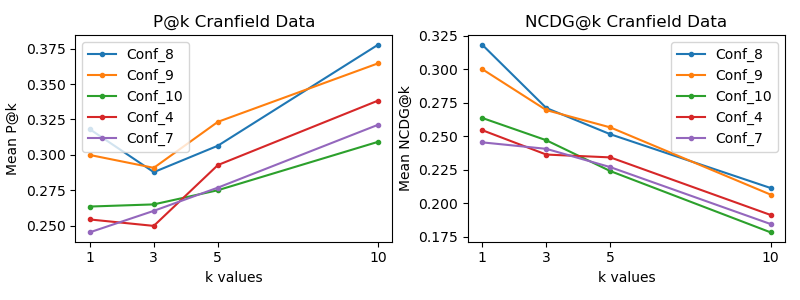
\includegraphics[scale=.85]{CranPlot.png}
\captionof{figure}{P@k and NCDG@k Plot Results for Cranfield Dataset}
\end{center}

If we were to choose the best Search Engine solely based on the NCDG@k curve we would choose the configuration for which this ratio is highest when k is maximal. Therefore, based on the previous plot, the champion configuration would be \textbf{Conf 8} (Stemming Analyzer \& BM25F).

\subsection{Time Dataset:}

We will follow the same structure and order to present the Time Dataset results:

\begin{table}[H]
\centering
\resizebox{\textwidth}{!}{%
\begin{tabular}{|p{1cm}|p{10cm}|p{10cm}|}
\hline
\textbf{Conf. ID} & \textbf{Text Analyzer}                & \textbf{Scoring Functions}  \\ \hline
1 & RegexTokenizer() $|$ LowercaseFilter() $|$ StopFilter(stoplist = STOP\_WORDS)              & scoring.TF\_IDF()            \\ \hline
2 & RegexTokenizer()$|$ StopFilter(stoplist = STOP\_WORDS) $|$ LowercaseFilter() $|$ StemFilter() & scoring.BM25F(K1=1.2, B=.75) \\ \hline
3               & StemmingAnalyzer(stoplist=STOP\_WORDS) & scoring.TF\_IDF()            \\ \hline
4               & FancyAnalyzer()                        & scoring.BM25F(K1=2, B=.8)    \\ \hline
5               & SimpleAnalyzer()                       & scoring.TF\_IDF()            \\ \hline
6               & StandardAnalyzer()                     & scoring.Frequency()          \\ \hline
7               & FancyAnalyzer()                        & scoring.BM25F()              \\ \hline
8               & StemmingAnalyzer(stoplist=STOP\_WORDS) & scoring.BM25F()              \\ \hline
9 & RegexTokenizer()$|$ StopFilter(stoplist = STOP\_WORDS) $|$ LowercaseFilter() $|$ StemFilter() & scoring.BM25F(K1=2, B=.8)    \\ \hline
10              & SimpleAnalyzer()                       & scoring.BM25F(K1=1.2, B=.75) \\ \hline
11              & StemmingAnalyzer(stoplist=STOP\_WORDS) & scoring.BM25F(K1=2, B=.8)    \\ \hline
12              & FancyAnalyzer()                        & scoring.TF\_IDF()            \\ \hline
\end{tabular}}
\caption{Configuration Overview for Time Dataset}
\label{tab:my-table}
\end{table}

\begin{table}[H]
\centering
\begin{tabular}{|c|c|c|c|c|c|c|c|}
\hline
\multicolumn{1}{|l|}{\textbf{Conf. ID}} &
  \multicolumn{1}{l|}{\textbf{MRR}} &
  \multicolumn{1}{l|}{\textbf{Mean}} &
  \multicolumn{1}{l|}{\textbf{Min}} &
  \multicolumn{1}{l|}{\textbf{1st Quartile}} &
  \multicolumn{1}{l|}{\textbf{Median}} &
  \multicolumn{1}{l|}{\textbf{3rd Quartile}} &
  \multicolumn{1}{l|}{\textbf{Max}} \\ \hline
11 & 0.725 & 0.555 & 0.000 & 0.264 & 0.539 & 0.906 & 1.000 \\ \hline
8  & 0.717 & 0.562 & 0.000 & 0.200 & 0.564 & 1.000 & 1.000 \\ \hline
2  & 0.708 & 0.557 & 0.000 & 0.200 & 0.564 & 1.000 & 1.000 \\ \hline
9  & 0.703 & 0.550 & 0.000 & 0.200 & 0.539 & 0.906 & 1.000 \\ \hline
4  & 0.689 & 0.539 & 0.000 & 0.200 & 0.500 & 0.889 & 1.000 \\ \hline
7  & 0.678 & 0.549 & 0.000 & 0.321 & 0.500 & 0.889 & 1.000 \\ \hline
10 & 0.669 & 0.542 & 0.000 & 0.321 & 0.500 & 0.889 & 1.000 \\ \hline
1  & 0.590 & 0.351 & 0.000 & 0.000 & 0.376 & 0.600 & 1.000 \\ \hline
3  & 0.566 & 0.309 & 0.000 & 0.000 & 0.333 & 0.500 & 1.000 \\ \hline
12 & 0.536 & 0.285 & 0.000 & 0.000 & 0.171 & 0.510 & 1.000 \\ \hline
6  & 0.457 & 0.238 & 0.000 & 0.000 & 0.063 & 0.500 & 1.000 \\ \hline
5  & 0.240 & 0.084 & 0.000 & 0.000 & 0.000 & 0.125 & 1.000 \\ \hline
\end{tabular}
\caption{MRR and R-Precision Overview for Time}
\label{tab:my-table}
\end{table}

\begin{center}
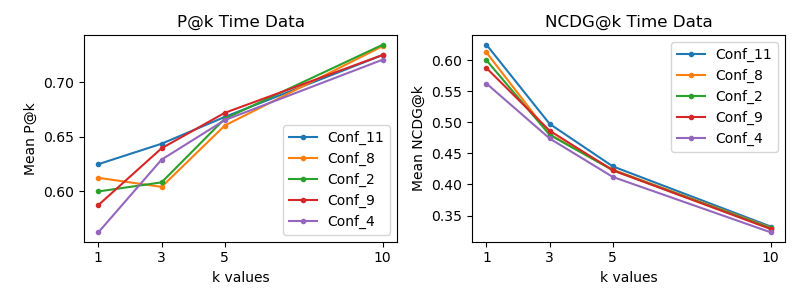
\includegraphics[scale=.85]{TimePlot.png}
\captionof{figure}{P@k and NCDG@k Plot Results for Time Dataset}
\end{center}

\section{Part 1.2}

To select the best Search-Engine modules for the “AwesomeSocialApp”, we will use the following evaluation metrics for ranking problems:

\textbf{Precision\@k:} If we consider ‘of all the query results we predicted to be True, how many were actually True?’ The graph shows that SE1 performs slightly better than SE3 and much better than SE2

\begin{center}
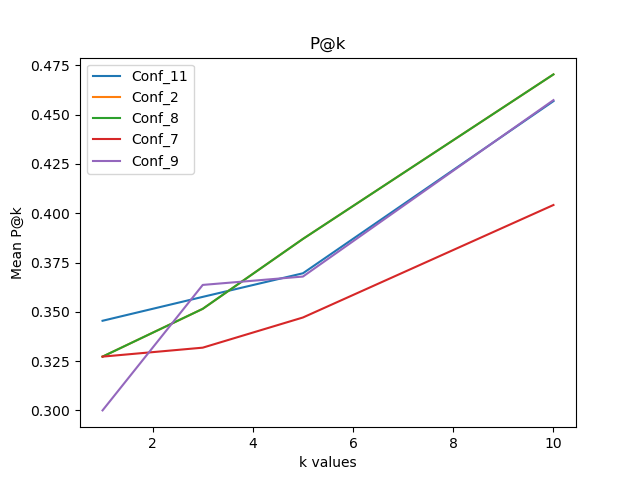
\includegraphics[scale=.25]{Pk.png}
\captionof{figure}{P@k Evaluation Metrics of Search Engines}
\end{center}

\textbf{Recall\@k:} If we consider ‘of all the query results that were actually True, how many I predicted to be True’. As we can see on graph below, SE3 should be selected compared with SE1 and SE2

\begin{center}
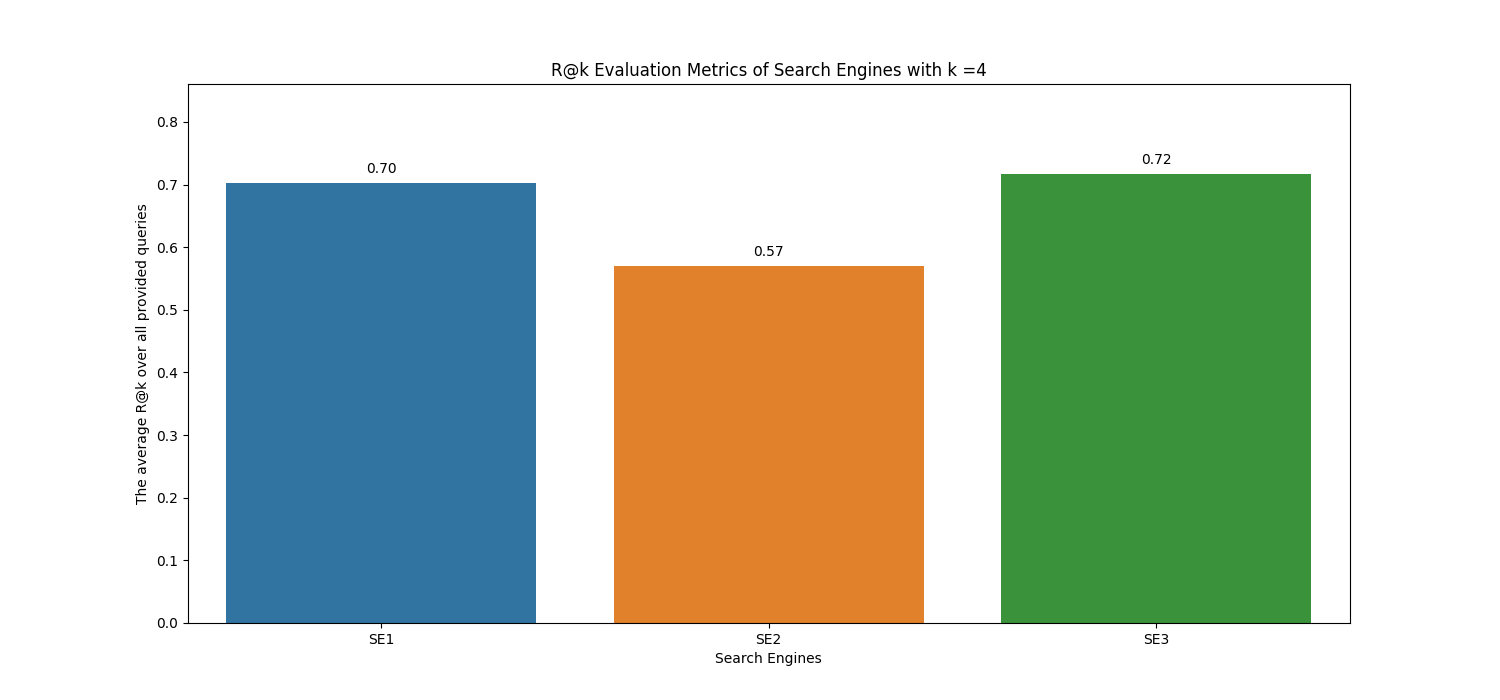
\includegraphics[scale=.25]{Rk.png}
\captionof{figure}{R@k Evaluation Metrics of Search Engines}
\end{center}

\textbf{NCDG\@k:} Normalized Discounted Cumulative Gain is a metric that is particularly good at evaluating search engines which return ranked outputs (the order of the output is relevant for this metric)

\begin{center}
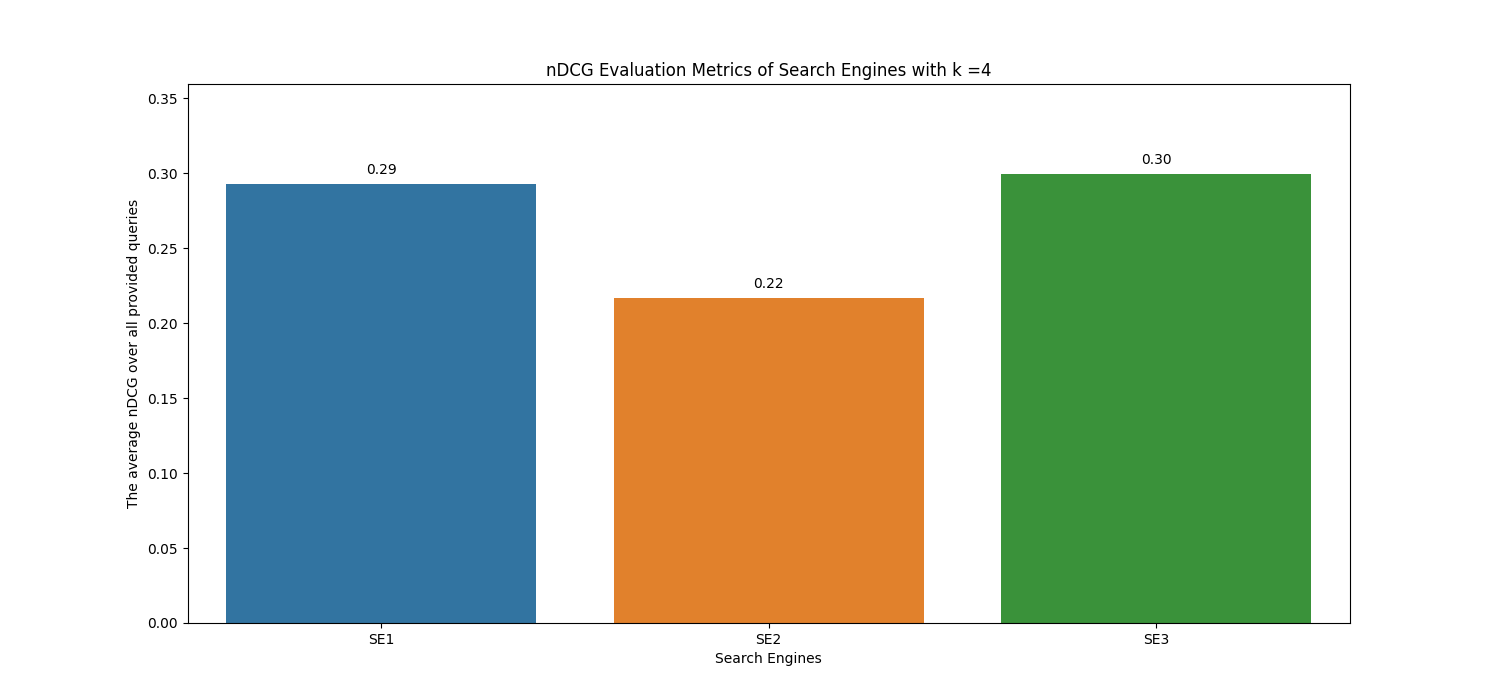
\includegraphics[scale=.25]{nDCG.png}
\captionof{figure}{nDCG@k Evaluation Metrics of Search Engines}
\end{center}

As we can see the figures on 3 graphs, SE1 and SE3 have a similar performance and much better than SE 2. But SE3 have a better performance on \textbf{nDCG@k} and \textbf{Recall@k} evaluation metrics, we highly recommend The “DummyDataScience” company to choose \textit{SE3} for this application.

\section{Part 2.1}

The first thing we have to do before running the LSH algorithm is to figure out the best $r$ (number of rows in each band), $b$ (number of bands) and $n$ (number of hash functions used) parameters such that we can minimize the number of False Positives and False Negatives. In particular, the choice of parameters will mainly help us to minimize the quantity of False Negatives. For the parameter choices we also need to take into account the following constraints:

\begin{equation}
r \cdot b = n
\end{equation}


\begin{equation}
0.97 > 1 - (1-0.95^r)^b
\end{equation}

From the second constraint, solving for b we can see that the following relation holds:

\begin{equation}
b > \frac{log(1-0.97)}{log(1-0.95^r)}
\end{equation}

Therefore, to minimze the False Negatives we will stress the $0.97$ bound as much as possible, specifically up to $0.999$. This will reduce the number of False Negatives, but will of course increase the number of False Positives. Since we will be able to remove some of the False Positives later on we are willing to make this compromise. So finally, fixing a value of $r=15$ we have decided to use the following parameters:

\begin{table}[H]
\centering
\begin{tabular}{|l|l|}
\hline
\textbf{r} & 15    \\ \hline
\textbf{b} & 12   \\ \hline
\textbf{n} & 180 \\ \hline
\end{tabular}
\caption{Parameter Overview}
\label{tab:my-table}
\end{table}

\begin{center}
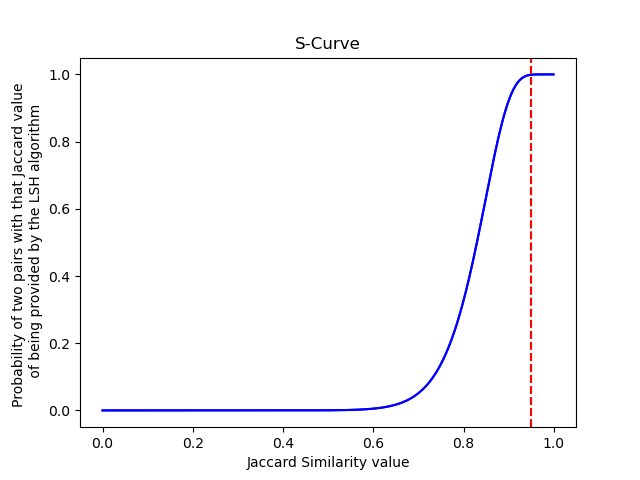
\includegraphics[scale=.70]{Splot.png}
\captionof{figure}{Relationship between Jaccard Similarity and probability that LSH will return that pair as a potential near duplicate}
\end{center}

After running the LSH algorithm with the previous set of parameters we got the following number of \textit{potential} near duplicate matches: \textbf{34655}. However, as we already mentioned before, we can still reduce the number of False Positives a posteriori by computing the Jaccard Similarity over the set of pairs provided by the LSH tool, and therefore eliminating those pairs which we will not be consider as near duplicates. For this purpose we have used the code named "False Positive Reduction" (in which we re-compute the real Jaccard similarity and not the approximated one), after which the number of \textit{final} near duplicates is: \textbf{33868}.

The total time required to run the LSH tool with the parameters highlighted previously was of \textbf{7 minutes and 15 seconds} on our machine.


\end{document}